%% $RCSfile: using.tex,v $
%% $Revision: 1.1 $
%% $Date: 2010/04/23 01:57:05 $
%% $Author: kevin $
%%
\chapter{Literature Review}\label{C:background}
\section{Background}

This chapter begins by providing a fundamental background to the field of server consolidation in Section \ref{}, then addresses several areas of current research interest.
Section \ref{} discusses the resource allocation in PaaS as well as the bi-level optimization including both biologically and non-biologically
inspired approaches; Section \ref{} delves into approaches that optimize the static placement. In addition, time-series aware problems and their approaches will be discussed; Section \ref{} discusses the issue of dynamic server consolidation and genetic programming; Section \ref{} covers approaches of scalability; Finally, Section \ref{} presents a summary of the important points identified in this review, alongside a discussion of the limitations of existing approaches.

\subsection{An Overview of server consolidation}







The reasons for energy wastage can be derived from several components of a data center, including 
cooling systems, network equipments, and server consumption. 
% A well-accepted measurement: PUE (Power Usage Effectiveness) \cite{Belady:IMLoaM62}
% a standard measurement for data center energy efficiency which compares the 
% total power with the power used to power IT equipment (e.g. server, network equipments). 
A recent survey \cite{Cho:2016kz} shows that the recent development of cooling techniques 
have reduced its energy consumption and now 
server consumption has become the dominate energy consumption component.
Despite improvements in hardwares, various software techniques have been proposed 
to reduce the energy consumption of servers 
such as: Server Consolidation and Dynamic Voltage and Frequency Scaling (DVFS) \cite{}.

% Virtualization \cite{Uhlig:2005ub} is the core technology that not only enables 
% the elastic management of Cloud resource but also can be used to improve the utilization and reduce 
% energy consumption.
% It maps a physical machine's system resource - including processors, memory, and 
% other devices - into isolated units called \emph{Virtual Machines (VMs)} which allows 
% multiple operating system to run on. 
% In essence, virtualization add an extra layer of software called 
% \emph{Virtual Machine Monitor (VMM)} or \emph{hypervisors} that can deploy, 
% release and migrate VMs at runtime. 
% Numerous VMMs have been designed for x86 commodity machines such as 
% Xen \cite{Barham:2003vu}, KVM \cite{Kivity:2007wu}, and VMware ESX server \cite{Barham:2003vu}.
 
% \textcolor{Maroon}{A brief introduction of server consolidation}

% It aims at improving the income by guaranteeing \emph{Quality of Service (QoS)}
% \cite{Calheiros:2011ul} of the maximum number of applications that a datacenter can accommodate.
Server consolidation \cite{Zhang:2010vo} is one of the widely used strategies 
for resource management \cite{marinescu2013cloud}.
It reduces the server energy consumption by gathering virtual machines (VMs) into a fewer 
number of physical servers so that idle servers can be turned off. 
The server consolidation techniques on the server-level
have been extensively studied in the past decade \cite{}. 
However, the recent development of container technology enables a VM-level of consolidation, which 
has not driven much attention. 
Container is a lightweight virtualization
technology which allows an application running in a single container. 
Multiple containers can be packed in a single virtual machine. 
Two main advantages make the container popular. 
First, containers do not need a Virtual Machine Monitor (VMM) but relies on the operating system; 
it reduces the overhead used on managing the virtual system. 
Second, the communication \cite{} between containers are much 
easier (e.g. inter-process communication) than an inter-VM communication. This feature is 
particularly useful for micro-service-based Web applications where their processes are packed
into separated containers.
This new technology has brought new challenges to server consolidation. 
Traditional algorithms can not be directly applied since there is an extra level
of virtualization. Affinity and communication aware allocation play an much important role 
in container-based environment. Therefore, new techniques and algorithms are need to be proposed. 

% Currently, few literatures address the 

% Therefore, this thesis will focus on providing solutions to 
% container-based server consolidation.

% Mainly, there are two types of method: static and dynamic.
% Static methods are often treated as off-line approaches and applied in a periodical manner 
% where a batch of VMs are allocated to a set of servers. 
% They are conducted at a given point of time when
% the overall utilization in a data-center is degraded into a certain level: 
% e.g, a predefined CPU utilization threshold. Because static methods often consider partial or all VMs
% in a datacenter, it is often treated as a global optimization task \cite{}.
% The static method often models the problem as a off-line bin-packing problem and 
% solved with deterministic or heuristic algorithms. The goal is often to find a global optimal solution
% in terms of server utilization and other criteria.
% Dynamic method is an on-line approach. It assumes a scenario when a single server is 
% overloading with multiple VMs, migrate one of the internal VMs out from 
% the host will release the overloading. Dynamic method is used in between 
% two static consolidation processes to ease the overloaded server as well as consolidation.
% As it only moves one VM at a time, it often applies greedy-based heuristic, therefore, hard to 
% reach a global optimization.

% \textcolor{Maroon}{Difficulty of server consolidation}
Server consolidation is often considered as 
a global optimization problem where its goal is to minimize the energy consumption.
Challenges are posed at different stages of consolidation process. 
Static problem is often modeled as a bin-packing problem  \cite{Mann:2015ua} 
which is known as NP-hard meaning it is unlikely to find an optimal solution 
of a large problem. 
Furthermore, server consolidation often has 
much complicated assumptions and constraints - including multi-dimension resources, 
migration cost, and heterogeneous bins \cite{Mann:2015ua}.
Because of its NP-hard nature, deterministic methods such as 
Integer Linear Programming \cite{Speitkamp:2010vp} and Mixed
Integer Programming \cite{} are unsuitable for a large scale problem 
because of the long computation time. 
Heuristic methods such as First Fit Decreasing (FFD) \cite{Panigrahy:2011wk}, 
Best Fit Decreasing (BFD) \cite{Xu:2010vh}, 
and other bin packing algorithms are often applied to approximate the optimal solution.
% Moreover, manually designed heuristics are designed to tackle the special requirements such 
% as \cite{}. 
% Although these greedy-based heuristics can quickly solve the consolidation problem, 
As \cite{Mann:2015ua} shown, server consolidation is a lot more harder than bin-packing problem,
therefore, these greedy-based heuristics can not reach a good approximation but easy to 
be stuck at a local optima.

% In addition to traditional VM-based server consolidation, container-based server consolidation
% has an extra level of virtualization which leads to an even difficult problem.
% Traditional server consolidation algorithms cannot be directly applied to 
% the problem because of the different structure and complexity. 

This thesis, therefore, aims at
providing an end-to-end solution to the container-based server consolidation problem.

% First, aggressive consolidation causes overloading physical resources. 
% It leads to performance degradation since the application cannot obtain enough resources
% the VM promised. It is hard to determine the maximum level of utilization of a physical machine.


Resource allocation and scheduling is the core of resource management in Cloud computing.
The main purpose is to satisfy both Cloud users' and Cloud providers' requirements by 
allocating sufficient resources to incoming tasks as well as keep a high utilization of the resources.
In order to accomplish this goal, 
resource allocation and scheduling tasks are often treated as optimization tasks.

An abstract model of resource allocation is shown in Figure \ref{}.





\subsection*{An Overview of Server Consolidation}

A Service consolidation is the process of packing virtual machines in a number of physical 
machines in order to reach a high utilization of resource as well as using a minimum number of 
physical machines. The key aspect of server consolidation is that, in order to achieve the 
desired result, the permutation of virtual machines must be considered. It is important to list the 
difference between a static and dynamic server consolidation approaches \cite{}. 
Static 
In static approaches, . In dynamic approaches, bla.... A typical system model for a data center
resource management system can be seen in Figure \ref{}. 
\begin{figure}
	\centering
	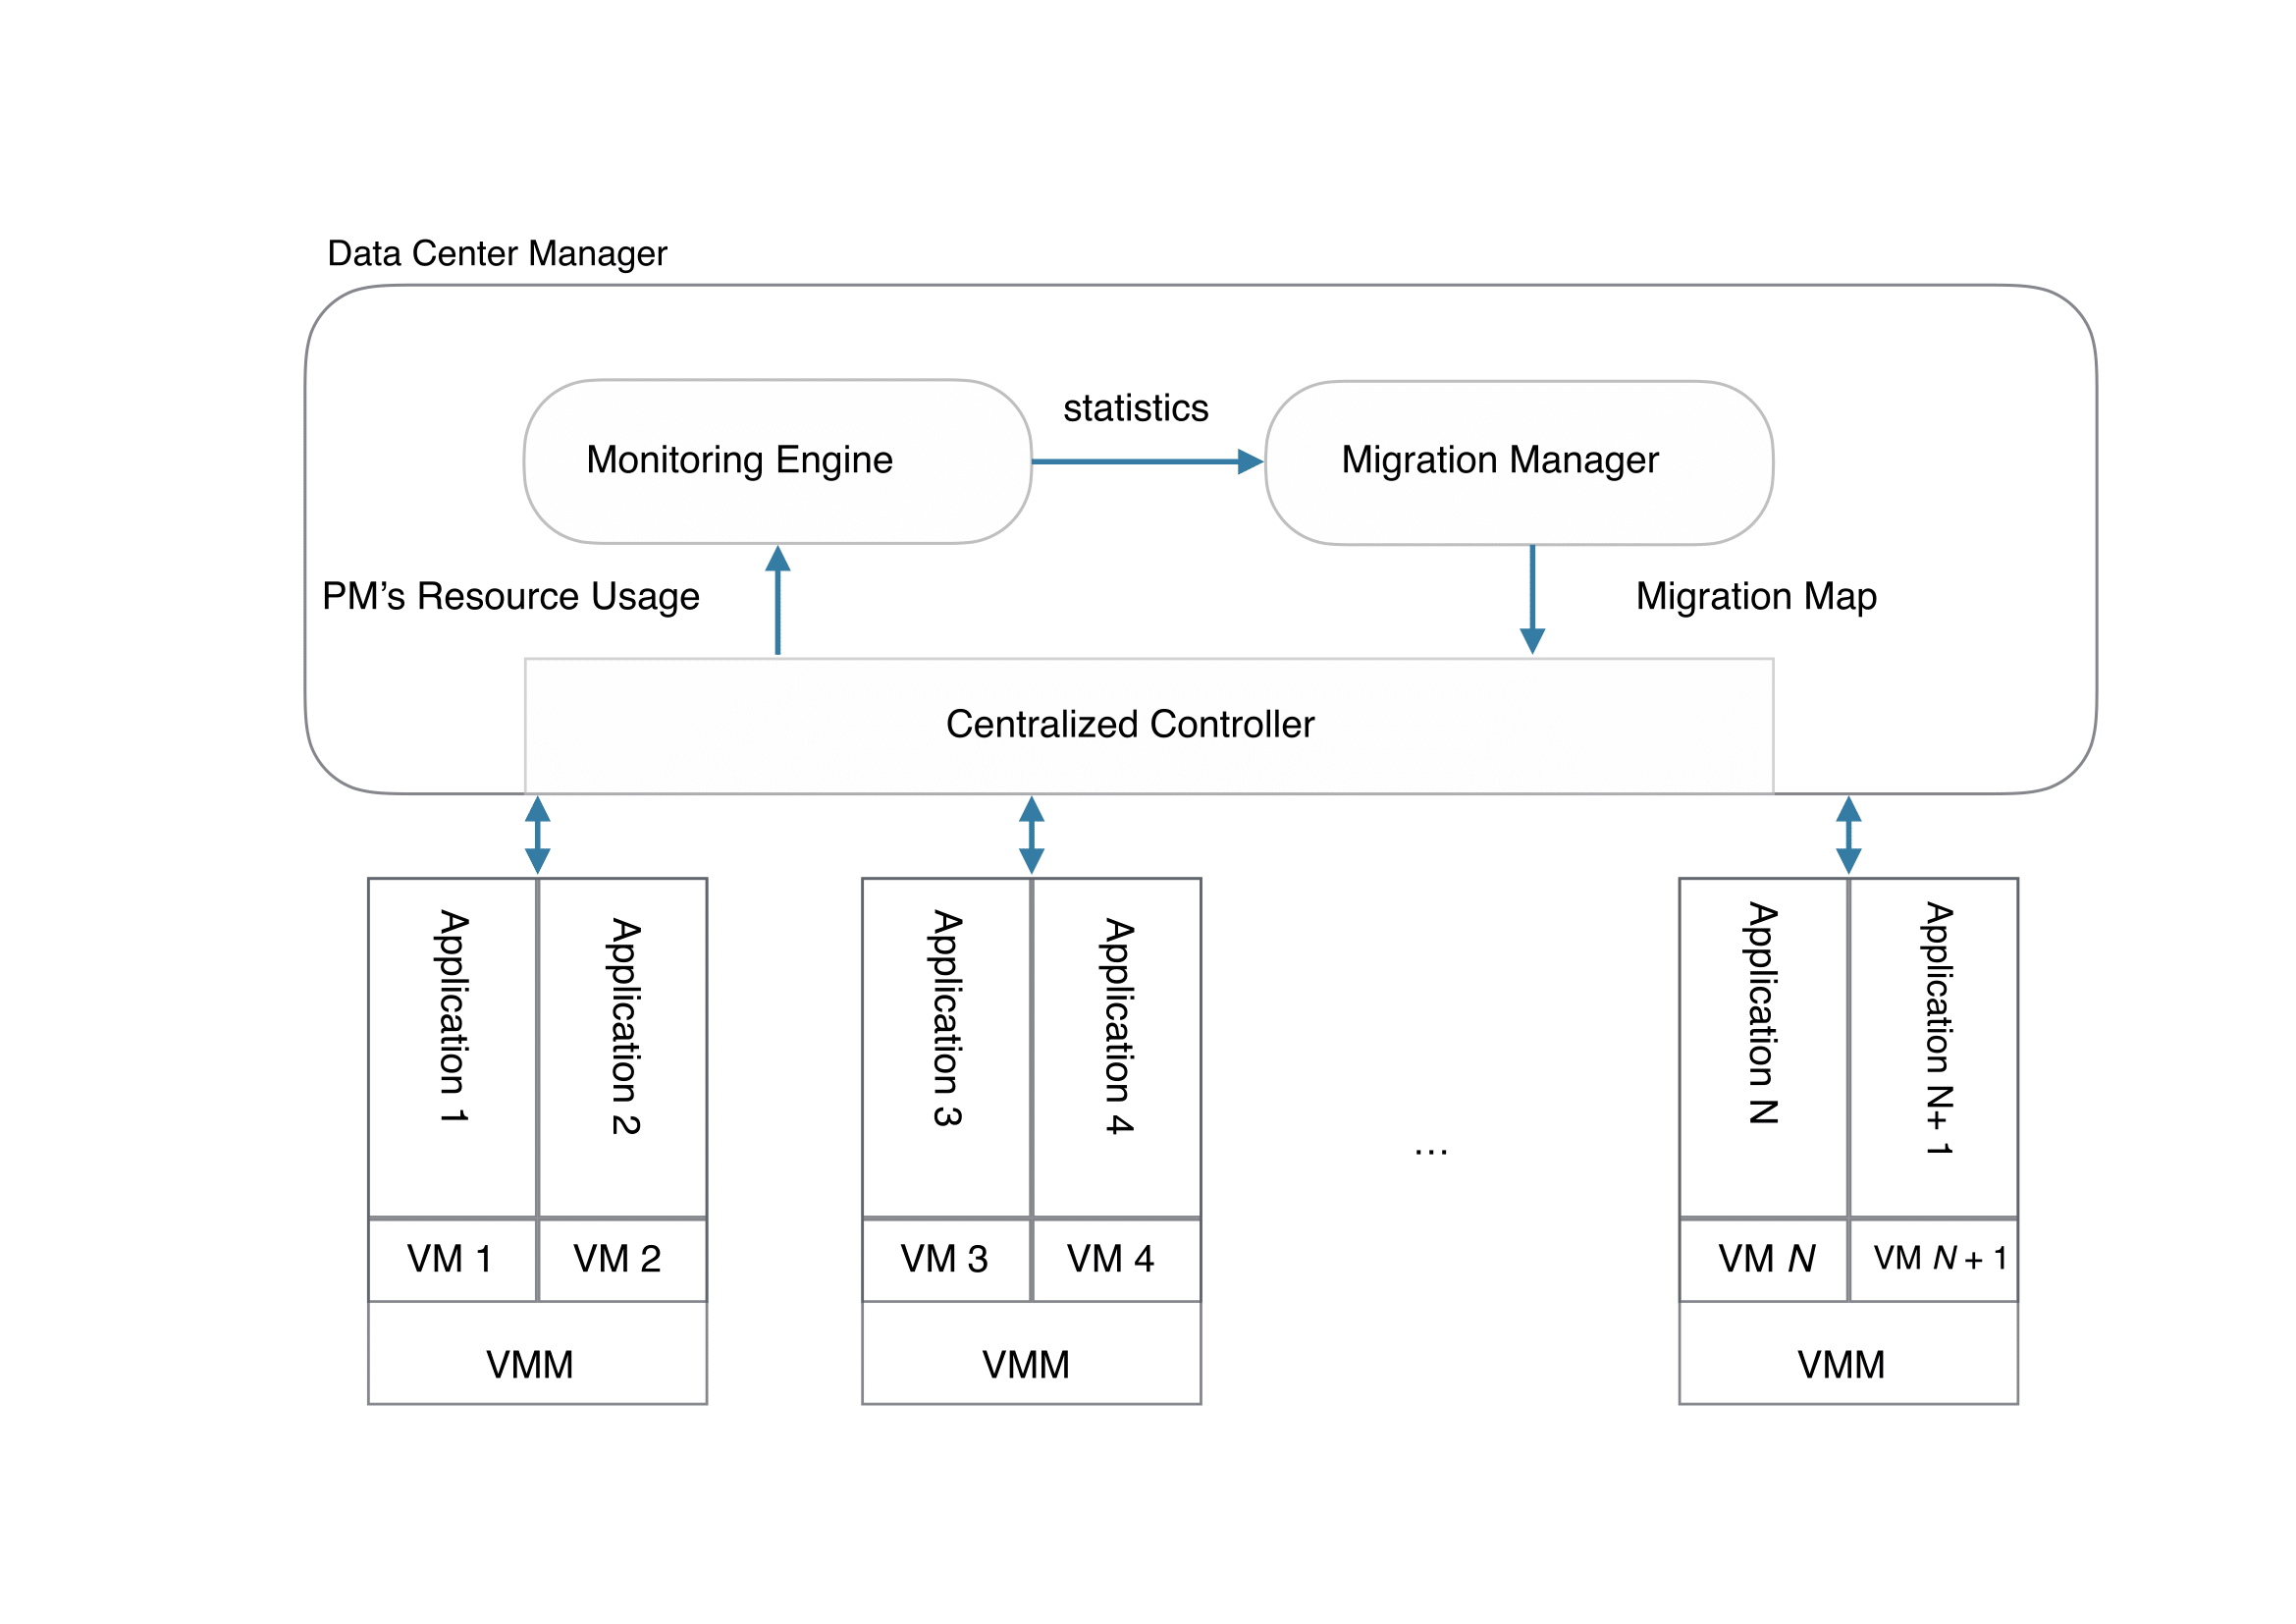
\includegraphics[width=1.0\textwidth]{pics/dataCenter-1.png}
	\caption{A datacenter management model \cite{Varasteh:2015fu}}
	\label{fig:arch}
\end{figure}

The taxonomy of server consolidation has not reach an agreement. In Verma's work \cite{Verma:2009wi}, they categorize it into three groups: static, semi-static and dynamic consolidation. In static consolidation, applications are placed on PM without any further movement. Semi-static refers to periodical adjustment. Dynamic consolidation is still applied on a set of VMs in response to their workload variations.









A dynamic server consolidation approach
can usually be decomposed into a series of steps, 
reflecting the process required to produce a solution \cite{}. 
These steps are shown in Figure \ref{} and discussed below:
\begin{enumerate}
	\item When to migrate. Dynamic migration occurs on two scenarios: migrating VMs from overloaded server; and item migrating VMs from underloaded server.
	\item Which VMs to migrate.  After deciding to migrate a VM from a server, the next step is 
	to make a decision of which VM to migrate.
	\item Where to migrate the VMs. The key step is to determine where to allocate a VM which leads to global optimization.
\end{enumerate}


\subsection*{A Comparison between CaaS and IaaS based Cloud model}
From a computing system design point of view, we believe service allocation and VM Placement
are closely related and should be considered as a single allocation task.
\subsection*{Service Allocation}
Service allocation refers to the process of mapping a Web service on a certain type of VM.
It is conducted by Cloud customers (e.g Web service providers) or Cloud brokers deligated by a 
Cloud customer.
The resource mapping involve with two steps, 
resource demand profiling \cite{} and VM selection \cite{}. 
Resource demand profiling is an estimation of the workload of a service. 
Because the web application has dynamic workload over time \cite{}, 
service providers or cloud brokers normally would like to estimate the future workload so that they 
can choose how much resources to rent in order to guarantee the 
Service Level Agreements (SLAs)  \cite{} to end customers. In this step, historical statistics
are often used and based on its peak workload estimation, service providers often
rent resources more than they need. Since the peak workload only accounts for a small portion
of its total operation time, intelligent strategies are applied to tackle the over-provisioning and 
under-provisioning problems.

Public Cloud providers often provide various configurations of VM, 
often refered to as VM types or instance types \cite{Li:2011ti}. 
An instance type is defined as its resources such as memory size, number of processors and 
CPU frequency. 

Previous research focus on how to rent an appropriate amount of resources so that it minimize the 
service providers' costs.

Ref \cite{Candeia:2010wt} considers e-Science applications with bag-of-tasks (BoT) model. It
aims at executing a bag of independent tasks with the least amount of Cloud resources before
a deadline.
Unlike a service allocation problem, where service is permanantly deployed in a reserved VM, 
they consider an on-demand VM allocation. 
That means, when a bag of tasks comes, the system
dynamically assign a set of VM to execute these tasks. 
It evaluates four heuristic algorithms and 
concludes that a greedy-based approach achieves the best result.

Li et al \cite{Li:2011ti} consider a dynamic cloud scheduling problem 
from Cloud brokers' perspective. It considers scenarios such as Cloud provider changing its offer 
(e.g changing of pricing schemes or VM types) and service performance changing, 
a cloud broker needs to adjust the VMs allocation across multiple Cloud providers. 
This work proposes a model which maximize a Cloud consumers' profit by adjusting VMs across
multiple Clouds. Their model does not consider a Cloud provider's profit.

Wang and Xia \cite{Wang:2016ui} propose a MIP formulation for energy-aware VM placement in Cloud.
The major difference between their work and previous work is that they use a non-linear energy model \cite{Gandhi:2009wp}.  Based on this model, they consider two resources CPU and memory. In order to solve the non-linear problem, they propose a linearization method which uses piecewise linear function to approximate the non-linear objective function. In the end, they uses a relaxation method to relax the integer linear programming problem into continuous and apply a rounding function to obtain a near-optimal solution. In summary, the energy model is the key objective in consolidation problem. With different models, the applied algorithm can be very different. However, EC approaches can deal with both linear and non-linear problem without any changes. That is an obvious advantage. 

% Virtualization technology was first developed in IBM System/360 in 1960s 
% targeting a finer granularity resource management. 
% It partitions a physical machine into separated resources 
% called virtual machine (VM) which can be allocated 
% and moved from one server to another. 
% This flexibility not only allows resources to be managed in a dynamic manner, 
% but also enables server consolidation.

% In a Cloud datacenter, server consolidation is used as technique to combat \emph{server sprawl}.
% Server sprawl refers to the low utilization of physical servers. The main cause for server sprawl is
% the requirement of running applications in isolation \cite{Vogels:2008bg}. 
% That is, an application is deployed in one or more servers which 
% offer much more resources than it needs. 
% With full virtualization \cite{}, a server's physical resources including CPUs, memory, and I/O devices
% are divided into finer granularity level of resources.
% Virtual machines offer different sizes of resources that 
% can be choosed to satisfy different demands from applications. 

\subsection*{An Overview of Evolutionary Computation}


\subsection*{Initial Placement}

\section*{Container-based VM Multiplexing}
Container has been introduced back in the 1980s' \cite{}. The recent development of container
allows only one process running in a container; this is revolutionary invention is called application
container. It plays an important role in Cloud computing since it is lightweighted, easier to configure
and enable finer adjustment than the VM-based resource management.


\begin{figure}
	\centering
	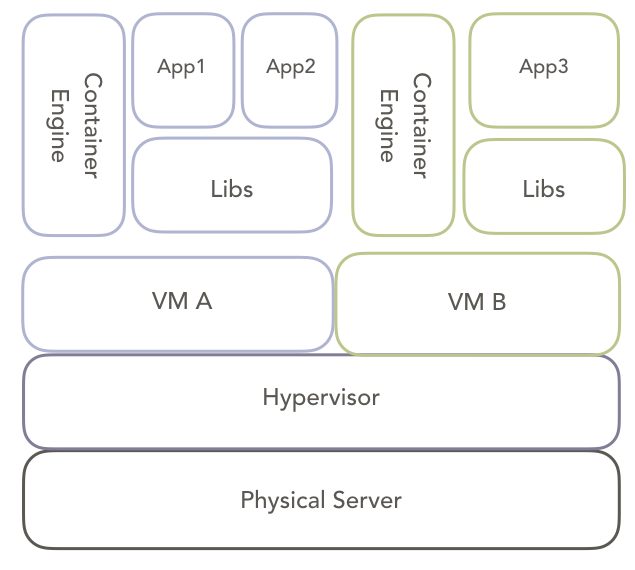
\includegraphics[width=0.6\textwidth]{pics/container.png}
	\caption{A Container as a Service Deployment Model}
	\label{fig:container}
\end{figure}

% % % % % \section*{Dynamic VM Placement}
% % % % The traditional dynamic VM placement approaches can be categorized into three groups: Heuristic
% % % based approaches, deterministic approaches and dyanmic techniques with load prediction.

% % However, we believe the dynamic VM placement problem is highly dependent on an overall workload

% \section*{Large scale VM Placement}
% If you are writing an MSc or PhD thesis you should \emph{not} be using this style. Instead use \verb=vuwthesis=, which is based on the book style, and conforms to the VUW thesis rules. The thesis style is rather different from the project report style. 

% This document is formatted using a local (to ECS and MSOR at VUW) style file. When you write your project report you should be very careful when changing the beginning. The document class settings should read:

% \begin{verbatim}
% \documentclass[11pt
%               , a4paper
%               , twoside
%               , openright
%               ]{report}
% \end{verbatim}
% The options to the document class specify that:
% \begin{itemize}
% \item 11pt font is to be used for the main body text,
% \item  we will print on A4 paper, 
% \item we will use duplex (two-sided) printing,
% \item we want chapters to start on a right-hand page. 
% \end{itemize}

% The opitons you supply to the  \texttt{vuwproject} style will depend upon
% what you are using the style for.

% \subsection{Specifying the details}
% The \texttt{vuwproject} style sets up the front page properly, and provides various commands allowing you to specify the author, title, supervisor or supervisors, the school from which the report is being submitted and the degree that the report is being submitted for. The style has deliberately been designed to do as little as possible. This means that your document can easily be re-formatted as a technical report, or for submission to a conference or journal by using the appropriate style.

% It is also possible to use the style to easily produce documents on a
% stand-alone computer where your \LaTeX installtion might not have all
% of the  files and fonts available to machines within ECS or MSOR.

% Most of the options to the \texttt{vuwproject} style are currently a simple
% choice and there's a default that will make it obvious if you do not make
% a choice.

% Use one of the following options to use fonts available on ECS/MSOR machines
% or to use images that imitate them (assumes you have copies of the images)
% \begin{itemize}
% \item \verb+font+
% \item \verb+image+
% \end{itemize}

% Use one of the following options to set the school,
% \begin{itemize}
% \item \verb+ecs+
% \item \verb+msor+
% \end{itemize}

% Use one of the following options to choose a pre-defined degree,
% \begin{itemize}
% \item \verb+bschonscomp+
% \item \verb+mcompsci+
% \end{itemize}

% or use this command to use an explicit degree or diploma name
% \begin{itemize}
% \item \verb+\otherdegree{DEGREE OR DIPLOMA NAME}+
% \end{itemize}

% So, for example, to submit a report for the Master of Comp Sci degree, which
% the style knows about, from within ECS, using the images, you'ld ensure the
%  \texttt{vuwproject} line options looked like:

% \begin{verbatim}
% \usepackage[image,ecs,mcompsci]{vuwproject}
% \end{verbatim}

% whereas for a degree from within MSOR, when creating the final version on
% an ECS or MSOR machine where you have access to the fonts, you would use
% these options

% \begin{verbatim}
% \usepackage[font,msor]{vuwproject}
% \end{verbatim}


% and add the other degree's name using this command 

% \begin{verbatim}
% \otherdegree{DEGREE OR DIPLOMA NAME}
% \end{verbatim}

% To specify the supervisor or supervisors use either of the following commands in the preamble.
% \begin{itemize}
% \item \verb+\supervisor{The Supervisor}+
% \item \verb+\supervisors{Super 1 and Super 2}+
% \end{itemize}

% If you fail to set any degree or supervisor, or the school, then the front page will report this.

% The \texttt{vuwproject} style also sets the default font to be Palatino, using the \texttt{mathpazo} package. Palatino is one of VUW's `offical' fonts, and is the font used for the heading on the front page. The \texttt{mathpazo} package also typesets maths in a style which suits Palatino. 

% \section{Copying the style}
% If you want to write your project report away from VUW you will need to make your own copy of the \texttt{vuwproject} style.

% You can find out where the original lives by reading the messages that \LaTeX\ prints when it is run.

% Alternatively, you can down load a copy of the  \texttt{vuwproject} style from
% the ECS webpages.

% Any changes made to your own copy of the \texttt{vuwproject} style will not be reflected in the original, and \textit{vice versa}. Hence it makes sense to leave this as it is, and use a local style file for your own definitions.   
